\documentclass[conference]{IEEEtran}
\usepackage[utf8]{inputenc}
\usepackage[english]{babel}
\usepackage{graphicx}
\usepackage{wrapfig}
\usepackage{graphics}
\graphicspath{ {images/} }
\usepackage{hyperref}
\usepackage{multicol}
\urlstyle{same}
\usepackage[ruled,vlined]{algorithm2e}
\begin{document}
\section{proposed solution}
in this paper we propose a solution for placement by combining two
other solutions, Genetic algorithm[1] and simulated annealing.
\subsection{simulated annealing}
simulated annealing is one of the most popular solution for the placement problem, it is an optimization solution that starts at initial state then start to choose a neighboring solution if it is better then replace the last solution with it.to use the simulated annealing we have to define the initial configuration.
\newline
\textbf{For initial configuration:} we will use a random placement for cells its coordinates is (x,y).
\newline
\textbf{For new configuration:} generate new circuit by placing the cells randomly.
\newline
\textbf{For initial temperature parameter:} we make it directly proportional to the number of cells in circuit, bigger number of cells higher temperature value.
\subsection{genetic algorithm}
genetic algorithm is taken out of the idea of "survival of the fittest", it's used in optimization as it uses the nature way of evolution like the fittest have the highest probability of survival, genetic algorithm chooses a random individual from population then make it the parent for the upcoming generation, and thus move towards the most optimal solution as show in figure[1].
.
 \begin{figure}[h]
    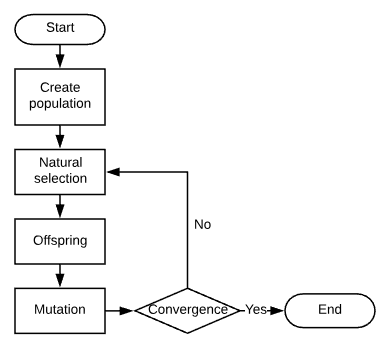
\includegraphics[width=0.5\textwidth]{images/gene.png}
    \caption{genetic algorithm}
\end{figure}
\newline
to use the genetic algorithm we have to form a population then produce children and do mutation .
\newline
\textbf{For population:} we will create the population out of simulated annealing solutions.
\textbf{For mutation:} we will swap two cells randomly.
\newline
\textbf{For offspring:} if the first parent have placement (x,y) and second parent placement is (z,k) then the child will have a placement like (x,k).
\subsection{proposed algorithm}
our proposed algorithm will combine the last two algorithms, by combining these algorithm we will generate some solutions by simulated annealing then use these solutions as population for the genetic algorithm, that will enhance the result of genetic algorithm as the population is no longer randomly generated but considers as optimized solution.
\newline
\newline
\textbf{algorithm steps}:
\begin{enumerate} 
\item generating some solutions (circuits) from simulated annealing.

\item use the simulated annealing solutions as genetic algorithm population.

\item use genetic algorithm to enhance the wire length.

\end{enumerate}

\begin{algorithm}
\SetAlgoLined
\KwResult{final placement }
 generate random placement (x,y) for cells\;
 \While{loop four times}{
 run simulated annealing and get a solution\;
 }
 create population for genetic out of the simulated annealing solutions\;
 \While{loop on population}{
  create the parents\;
  produce the children\;
  do the mutation\;
 }
 \caption{proposed algorithm}
\end{algorithm}
\subsection{Experimental and Comparison Studies}
in this section we will compare between the proposed algorithm and the simulated annealing and genetic algorithm.
for experiment we used a 10x10 grid and different cells numbers and population size = 4 for the genetic algorithm and the proposed algorithm.

\begin{table}[h!]
\centering
\begin{tabular}{ |c || p{1.5cm}|p{1.5cm}|p{1.5cm}|p{1.5cm}|}
 \hline
 number of cells & \multicolumn{4}{|c|}{Wire length} \\
 \hline
   & initial placement & simulated annealing & genetic algorithm & proposed algorithm\\
 \hline
 7 & 66 & 48 & 45 & 44 \\ [1ex] 
 \hline
 20 & 245 & 170 & 156& 151 \\[1ex] 
 \hline
 40 & 375 & 348 & 335 & 296\\[1ex] 
 \hline
 52 & 461 & 461 & 426& 394 \\ [1ex] 
 \hline
\end{tabular}
\caption{experiment results}
\label{table:1}
\end{table}
the results are dependent on the number of connections for the one cell, and not constants it depends on the run. However, with each run the proposed algorithm has the best results between the other two algorithm. \newline
the proposed algorithm has the best result and the shortest wire length,however it is slower than both algorithm as it needs the simulated annealing run at first multiple times then run the genetic algorithm.

\section{conclusion}
this paper propose a new algorithm for replacement by combining two other algorithms, the proposed algorithm have much better results compared with the other two, but needs more time.\newline for future work maybe we try finding a way to reduce the run time.
\section{references}
\begin{enumerate} 
\item A Genetic Algorithm for Macro Cell Placement, Henrik Esbensen*
,Computer Science Department Aarhus University DK-8000 Aarhus C, Denmark.

\end{enumerate}
\end{document}
